\section{Results} \label{sec:results}

%==============[	  Basket Trading  ]==============
Our pairs trading strategy represents a specialized implementation of basket trading, where a synthetic asset is constructed through an optimally weighted basket of securities. The strategy's feasibility rests on several key operational assumptions and market structure considerations that warrant careful examination. The basket's composition demonstrates sophisticated risk distribution across multiple market segments, with our synthetic control comprising 27 assets spanning diverse sectors. Significant long positions in AME (41.08\%), LUV (33.31\%), and TFC (25.60\%) are counterbalanced by strategic shorts in ADSK (-42.25\%) and UNP (-25.77\%), creating a well-diversified exposure structure that provides distinct advantages over traditional single-stock pairs.

This sophisticated composition yields multiple advantages through its sector diversity. By spanning financials, technology, transportation, and other sectors, our approach substantially reduces idiosyncratic risk compared to single-stock pairs, effectively mitigating the impact of company-specific events or sector-wide shocks that typically destabilize simpler pairs trading arrangements. The implementation efficiency is further enhanced by modern execution systems that can treat these 27 components as a single basket order, substantially reducing transaction costs and bid-ask spread impact through optimized order routing.

The practical implementation of this strategy requires careful consideration of several critical operational requirements. Most importantly, the approach necessitates access to sophisticated basket trading capabilities that can handle simultaneous execution of multiple components--a requirement readily met by major institutional brokers offering advanced smart order routing services. To ensure consistent execution quality, all basket components must maintain sufficient liquidity; we addressed this constraint by restricting our universe to S\&P 500 constituents, thereby guaranteeing deep and reliable trading volumes across all components.

The strategy's effectiveness ultimately depends on maintaining strict dollar neutrality through equal but opposite positions in the target and synthetic basket. This market-neutral construction demands precise execution coordination across all components, a challenge effectively addressed by modern electronic trading systems capable of processing complex basket orders as single units. 

%==============[	  Comments on Figure 5  ]==============
\cref{fig:positions_by_copula} illustrates the evolution of position sizes for both target and synthetic assets across different copula specifications over our out-of-sample period from July 2020 to January 2025. For each copula family, the strategy maintains dollar-neutral positions by simultaneously taking offsetting long and short positions in the target (red) and synthetic (blue) assets. Position sizes (in shares) are normalized relative to an initial equity of \$1, with values between -0.2 and 0.2 representing the number of shares allocated to each side of the trade. The parallel movements in the red and blue lines across all panels reflect the strategy's market-neutral construction, where positions are always equal in magnitude but opposite in direction.

%==============[	  Figure 5 ]==============
\inserthere{fig:positions_by_copula}
\begin{figure}[H]
  \caption{Position Sizes Over Time by Copula Family}
  \centering
  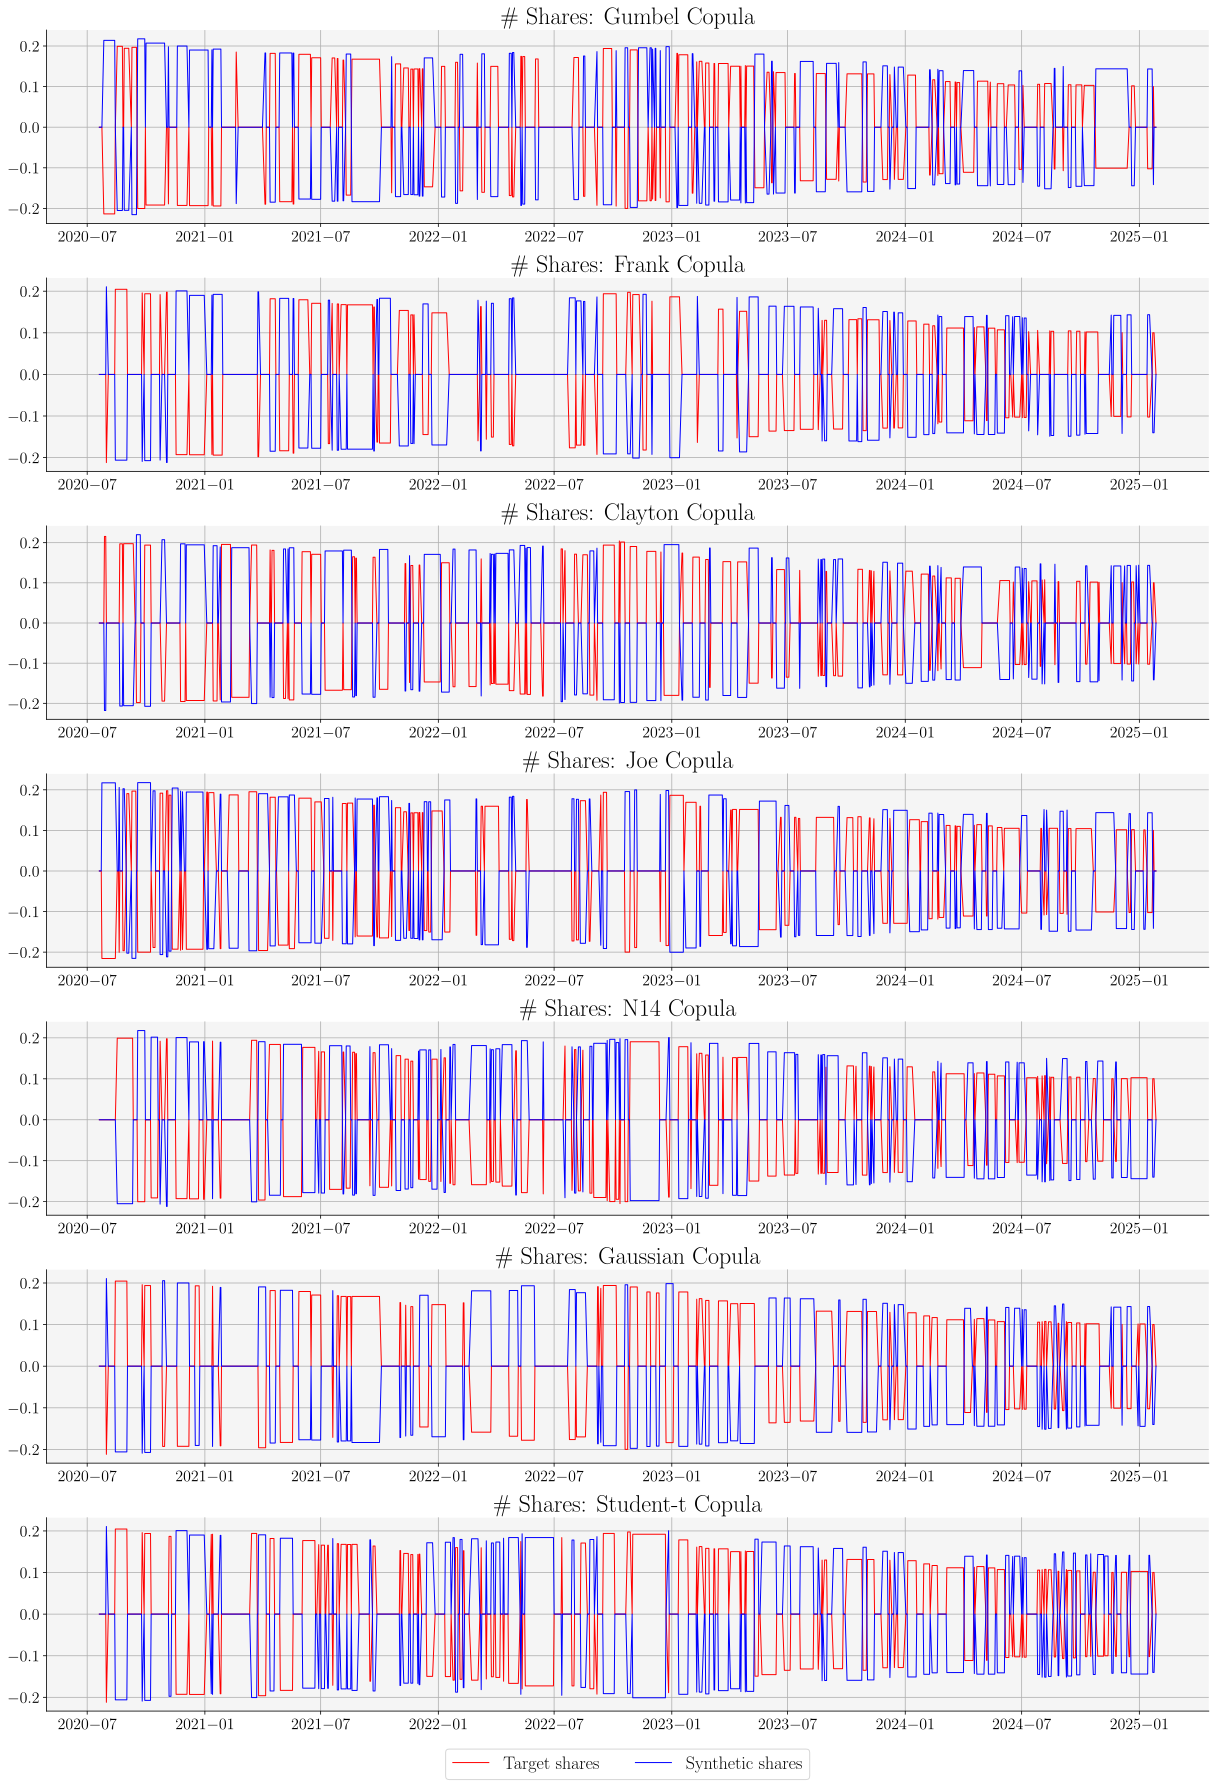
\includegraphics[scale=0.315]{/Users/jesusvillotamiranda/Library/CloudStorage/OneDrive-UniversidaddeLaRioja/GitHub/Repository/arbitragelab-master/__OUTPUT_TeX__/figures/positions_by_copula.pdf}
  \label{fig:positions_by_copula}
%.............
\vspace{0.2cm}
\begin{minipage}{\textwidth}
\setlength{\parindent}{0pt}
\small\textit{Note: 
This figure shows the evolution of position sizes (in shares) for target (red) and synthetic (blue) assets in the test sample under different copula specifications. The strategy assumes initial equity of \$1.
}
\end{minipage}
%.............

\end{figure}


\cref{tab:copula_performance} reveals the out-of-sample performance across copula specifications. The N14 mixed copula generates the highest total return (77.82\%) and annualized return (17.26\%), while maintaining moderate volatility (4.35\%). This superior performance is reflected in its high Sharpe (3.97) and Sortino (5.75) ratios, matching the Clayton copula's risk-adjusted metrics but with better absolute returns. The Gaussian copula, despite showing the most conservative returns (62.70\%), still achieves respectable risk-adjusted performance with a Sharpe ratio of 3.14, though it lags behind all other specifications.
A particularly noteworthy pattern emerges in the downside risk metrics. The Frank copula, while generating modest returns (66.53\%), exhibits the lowest volatility (3.97\%) and maintains a remarkably low maximum drawdown (1.36\%), suggesting it effectively filters out noisy trading signals. In contrast, the Joe copula shows the highest maximum drawdown (2.57\%) despite having the highest win rate (36.62\%), indicating that its emphasis on upper tail dependence may lead to larger adverse price movements before positions converge. The Student-t copula strikes a balance between these extremes, delivering strong total returns (74.63\%) with moderate maximum drawdown (2.15\%) and a competitive Sharpe ratio (3.60), demonstrating that its symmetric tail dependence effectively captures the risk-return tradeoff inherent in our pairs trading strategy.
%==============[	  Table 3 ]==============
\inserthere{tab:copula_performance}
\begin{table}[H]
\centering
\caption{Performance Metrics by Copula}
\label{tab:copula_performance}
\small\begin{tabular}{lR{1.2cm}R{1.2cm}R{1.1cm}R{1.3cm}R{1.3cm}R{1.3cm}R{1.2cm}R{1.2cm}R{1.2cm}R{1.3cm}}
\toprule
Copula & Total Return (\%) & Ann. Return (\%) & Ann. Vol. (\%) & Sharpe Ratio & Sortino Ratio & Calmar Ratio & Max DD (\%) & Win Rate (\%) & Profit Factor & VaR-95 (\%) \\
\midrule
Gumbel & 72.59 & 16.10 & 4.61 & 3.49 & 4.42 & 7.42 & 2.17 & 34.86 & 2.19 & -0.35 \\
Frank & 66.53 & 14.76 & 3.97 & 3.71 & 4.75 & 10.85 & 1.36 & 30.55 & 2.51 & -0.30 \\
Clayton & 74.67 & 16.56 & 4.18 & 3.97 & 5.30 & 10.89 & 1.52 & 32.31 & 2.60 & -0.31 \\
Joe & 67.45 & 14.96 & 4.62 & 3.24 & 3.85 & 5.83 & 2.57 & 36.62 & 2.02 & -0.36 \\
N14 & 77.82 & 17.26 & 4.35 & 3.97 & 5.75 & 11.25 & 1.53 & 34.07 & 2.50 & -0.32 \\
Gaussian & 62.70 & 13.91 & 4.43 & 3.14 & 4.10 & 8.12 & 1.71 & 32.31 & 2.07 & -0.35 \\
Student-t & 74.63 & 16.55 & 4.60 & 3.60 & 4.64 & 7.70 & 2.15 & 35.04 & 2.30 & -0.33 \\
\bottomrule
\end{tabular}

%.............
\vspace{0.5cm}
\begin{minipage}{\textwidth}
\setlength{\parindent}{0pt}
\small\textit{Note: 
This table reports various performance metrics for pairs trading strategies implemented using different copula specifications. Performance measures include total and annualized returns, annualized volatility, risk-adjusted ratios (Sharpe, Sortino, and Calmar), maximum drawdown (Max DD), win rate, profit factor, and 95\% Value-at-Risk (VaR-95). All metrics are computed over the out-of-sample period from July 2020 to January 2025.
}
\end{minipage}
%.............

\end{table}


%\begin{table}[H]
%\centering
%\caption{Performance Metrics by Copula}
%\label{tab:copula_performance}
%\small\begin{tabular}{lR{1.2cm}R{1.2cm}R{1.1cm}R{1.3cm}R{1.3cm}R{1.3cm}R{1.2cm}R{1.2cm}R{1.2cm}R{1.3cm}}
%\toprule
%Copula & Total Return (\%) & Ann. Return (\%) & Ann. Vol. (\%) & Sharpe Ratio & Sortino Ratio & Calmar Ratio & Max DD (\%) & Win Rate (\%) & Profit Factor & VaR-95 (\%) \\
%\midrule
%Gumbel & 72.59 & 16.10 & 4.61 & 3.49 & 4.42 & 7.42 & -2.17 & 34.86 & 2.19 & -0.35 \\
%Frank & 66.53 & 14.76 & 3.97 & 3.71 & 4.75 & 10.85 & -1.36 & 30.55 & 2.51 & -0.30 \\
%Clayton & 74.67 & 16.56 & 4.18 & 3.97 & 5.30 & 10.89 & -1.52 & 32.31 & 2.60 & -0.31 \\
%Joe & 67.45 & 14.96 & 4.62 & 3.24 & 3.85 & 5.83 & -2.57 & 36.62 & 2.02 & -0.36 \\
%N14 & 77.82 & 17.26 & 4.35 & 3.97 & 5.75 & 11.25 & -1.53 & 34.07 & 2.50 & -0.32 \\
%Gaussian & 62.70 & 13.91 & 4.43 & 3.14 & 4.10 & 8.12 & -1.71 & 32.31 & 2.07 & -0.35 \\
%Student-t & 74.63 & 16.55 & 4.60 & 3.60 & 4.64 & 7.70 & -2.15 & 35.04 & 2.30 & -0.33 \\
%\bottomrule
%\end{tabular}
%\end{table}

%\begin{table}[H]
%\centering
%\caption{Performance Metrics by Copula}
%\label{tab:copula_performance}
%\small\begin{tabular}{lR{1.2cm}R{1.2cm}R{1.1cm}R{1.3cm}R{1.3cm}R{1.3cm}R{1.2cm}R{1.2cm}R{1.2cm}R{1.3cm}}
%\toprule
%Copula & Total Return (\%) & Ann. Return (\%) & Ann. Vol. (\%) & Sharpe Ratio & Sortino Ratio & Calmar Ratio & Max DD (\%) & Win Rate (\%) & Profit Factor & VaR-95 (\%) \\
%\midrule
%Gumbel & 72.59 & 16.10 & 4.61 & 3.49 & 4.42 & 0.11 & -152.88 & 34.86 & 2.19 & -0.35 \\
%Frank & 66.53 & 14.76 & 3.97 & 3.71 & 4.75 & 0.48 & -30.92 & 30.55 & 2.51 & -0.30 \\
%Clayton & 74.67 & 16.56 & 4.18 & 3.97 & 5.30 & 0.17 & -98.60 & 32.31 & 2.60 & -0.31 \\
%Joe & 67.45 & 14.96 & 4.62 & 3.24 & 3.85 & 0.14 & -110.30 & 36.62 & 2.02 & -0.36 \\
%N14 & 77.82 & 17.26 & 4.35 & 3.97 & 5.75 & 0.41 & -42.44 & 34.07 & 2.50 & -0.32 \\
%Gaussian & 62.70 & 13.91 & 4.43 & 3.14 & 4.10 & 0.45 & -30.92 & 32.31 & 2.07 & -0.35 \\
%Student-t & 74.63 & 16.55 & 4.60 & 3.60 & 4.64 & 0.54 & -30.92 & 35.04 & 2.30 & -0.33 \\
%\bottomrule
%\end{tabular}
%\end{table}

\cref{fig:equity_curves_comparison} displays the cumulative returns for our pairs trading strategy across different copula specifications. The performance hierarchy is well-defined throughout the out-of-sample period: the N14 mixed copula consistently outperforms all other specifications, achieving approximately 78\% cumulative return. A second group comprising the Student-t, Clayton, and Gumbel copulas tracks closely together, delivering returns around 73-75\%. Joe and Frank copulas form a third tier with returns near 67\%, while the Gaussian copula lags notably behind all other specifications with about 63\% cumulative return. This ordering largely aligns with the sophistication of tail dependence modeling in each specification, suggesting that more flexible approaches to capturing the joint distribution of target and synthetic returns translate directly into superior trading performance.

%==============[	  Figure  ]==============
\inserthere{fig:equity_curves_comparison}
\begin{figure}[H]
  \caption{Equity Curves Comparison Across Copula Families}
  \centering
  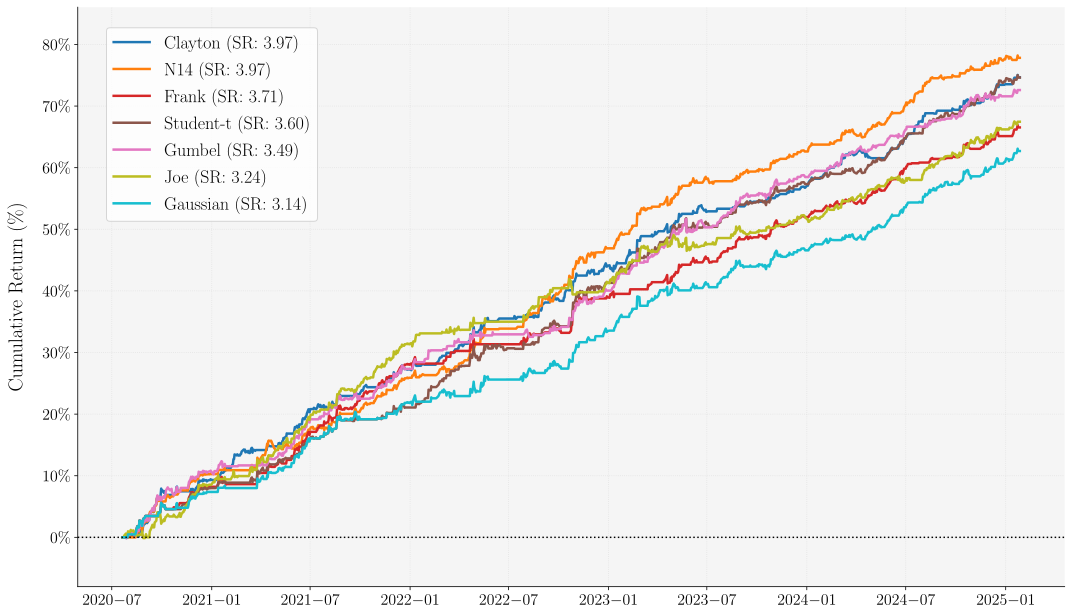
\includegraphics[scale=0.47]{/Users/jesusvillotamiranda/Library/CloudStorage/OneDrive-UniversidaddeLaRioja/GitHub/Repository/arbitragelab-master/__OUTPUT_TeX__/figures/equity_curves_comparison.pdf}
  \label{fig:equity_curves_comparison}
%.............
\vspace{0.5cm}
\begin{minipage}{\textwidth}
\setlength{\parindent}{0pt}
\small\textit{Note: 
This figure compares the cumulative returns of trading strategies based on different copula specifications in the test sample. Each line represents a different copula model, with their respective Sharpe Ratios (SR) shown in parentheses. The y-axis shows cumulative returns in percentage terms, and the x-axis displays the timeline in six-month intervals.
}
\end{minipage}
%.............

\end{figure}




\paragraph{Risk-adjusted returns}

For each copula model, we run the  regression
$$
\mathcal{R}_{t}^{c} = \alpha + \b{\beta}' \mbf{f}_t + \eps_t
$$
where 
$\mathcal{R}_{t}^{c}$ are the excess returns of our pairs trading strategy for copula family $c$, and 
$\mbf f_t$ represents a particular combination of the Fama-French factors: 
$\texttt{MKT\_RF}_t$, $\texttt{SMB}_t$, $\texttt{HML}_t$, $\texttt{RMW}_t$, $\texttt{CMA}_t$, $\texttt{MOM}_t$, $\texttt{ST\_REV}_t$, $\texttt{LT\_REV}_t$.
Since we consider combinations of 8 factors, we run $2^8=256$ different regressions for each copula. This delivers a positive significant $\alpha$ of  $0.0004$ -- $0.0006$ for all regressions specifications across all copula models, which is equivalent to an annualized $\alpha$ of $10.08\%$ -- $15.12\%$. The significance of risk-factors varies through copula models. In particular: 
%----------------------------------------------------
\begin{itemize}[leftmargin=*,noitemsep]
  \item Gumbel copula shows limited factor exposure, with only the Size (SMB) factor showing statistical significance and the Value (HML) factor showing mild significance. The Short-term Reversal (ST\_REV) factor exhibits mild significance, although the overall factor model reliability is questionable.
  
  \item Frank copula returns demonstrate significant exposure primarily to the Short-term Reversal (ST\_REV) factor, with other factors showing no consistent statistical significance.
  
  \item Clayton copula strategy returns are significantly exposed to market risk, with MKT\_RF being the sole statistically significant factor across all model specifications.
  
  \item Joe copula exhibits mild sensitivity to market risk, with MKT\_RF showing moderate significance. The single-factor model incorporating only MKT\_RF emerges as the most statistically significant specification.
  
  \item N14 copula returns show significant exposure to the market factor. The model's explanatory power improves notably when incorporating the Short-term Reversal factor.
  
  \item Gaussian copula demonstrates significant exposure to market risk, with the Short-term Reversal factor showing strong statistical significance (significant at the 1\% level). 
  
  \item Student-t copula returns exhibit mild sensitivity to the Profitability factor (RMW), suggesting the potential relevance of a single-factor model focused solely on RMW.
\end{itemize}
%----------------------------------------------------